Table~\ref{tab:params} shows that the main comparison keeps the trainable
parameter counts closely matched. The MLP uses 23 trainable parameters, while
the VQC uses 22.

\begin{table}[t]
  \centering
  \caption{Trainable parameter counts for the main L1 comparison.}
  \label{tab:params}
  \begin{tabular}{lrr}
    \hline
    Agent & Trainable parameters & All parameters \\
    \hline
    DQN-MLP & 23 & 23 \\
    DQN-VQC & 22 & 22 \\
    \hline
  \end{tabular}
\end{table}

\begin{figure}[t]
  \centering
  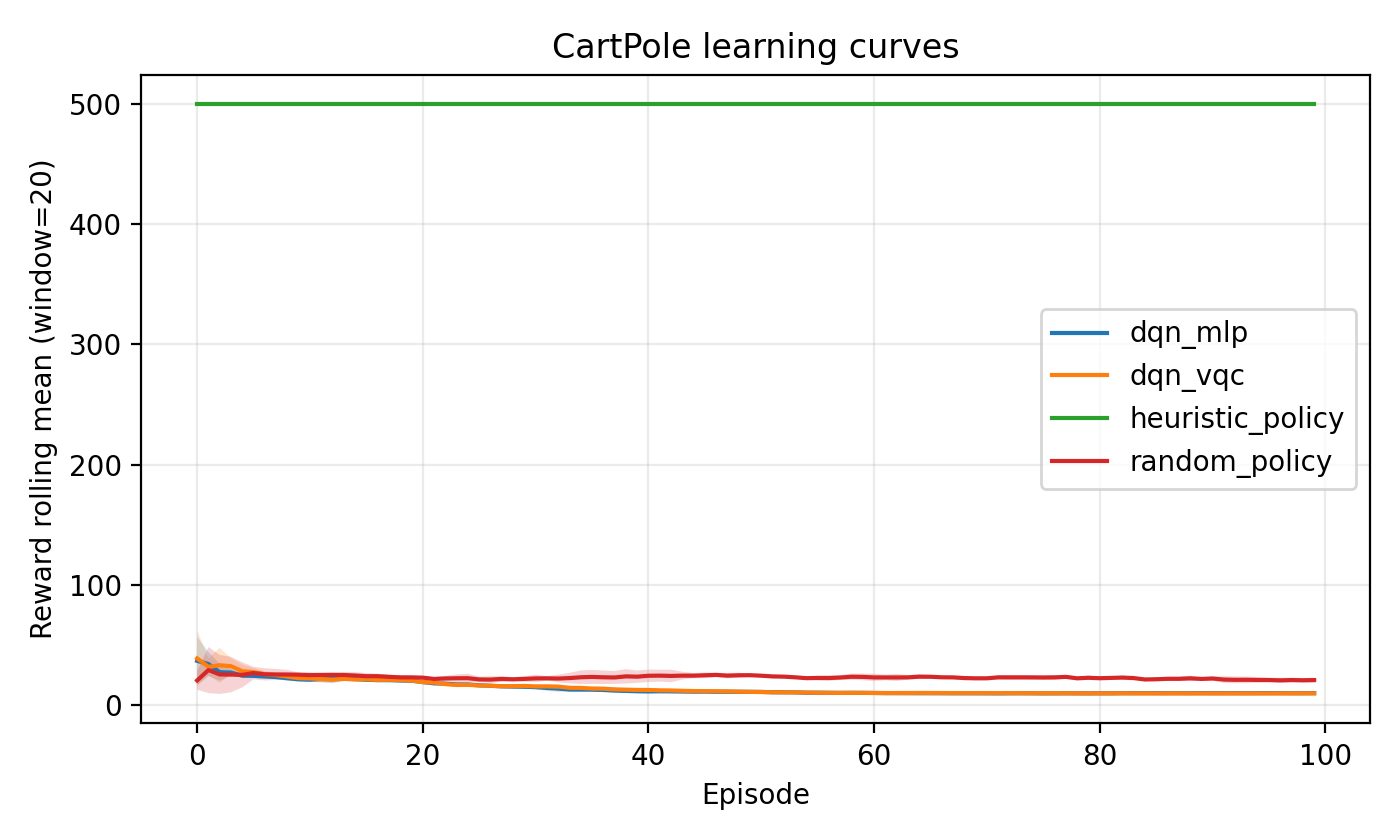
\includegraphics[width=0.95\linewidth]{figures/cartpole_l1_eval100_with_baselines.png}
  \caption{Learning curves on CartPole-v1 with random and heuristic reference policies.}
  \label{fig:learning-curve}
\end{figure}

Table~\ref{tab:results} summarizes the main results over 5 seeds for 100-episode
runs and 3 seeds for extended runs. Both learned agents score below the
random-policy baseline (20.65 $\pm$ 2.01): DQN-MLP at 9.42 $\pm$ 0.50 and
DQN-VQC at 9.42 $\pm$ 0.45. The near-identical scores and low standard
deviations indicate both collapsed to a single-action deterministic policy:
a constant-action policy survives approximately 9 steps, while a random policy
alternates actions and survives approximately 20 steps. Widening the epsilon
decay from 800 to 2000 steps (so $\epsilon$ never saturates during training)
did not change the collapse, ruling out exploration scheduling as the primary
cause. The heuristic controller (500.00) is a ceiling reference only.

Extended 500-episode training with proportional epsilon decay reveals seed
dependence: MLP seed 0 reaches greedy 69.45 (17,646 steps) while seeds 1--2
stay at $\approx$9.3. VQC seeds remain uniformly poor (9.65--13.95).

These results suggest that under the 22--23 parameter budget, final policy
quality is dominated by the exploration schedule, training length, and random
seed rather than by the classical-vs-quantum choice. Short training runs with
tight epsilon schedules are particularly fragile for small models.

\begin{table}[t]
  \centering
  \caption{Main CartPole-v1 results over 5 seeds (100-episode runs) and 3 seeds (500-episode runs). $\epsilon$ decay over 2000 steps for 100-ep runs, 4000 for 500-ep.}
  \label{tab:results}
  \footnotesize
  \begin{tabular}{lcccl}
    \hline
    Configuration & Params & Seeds & Greedy eval & Time (s) \\
    \hline
    Random & -- & -- & 20.65 $\pm$ 2.01 & -- \\
    Heuristic & -- & -- & 500.00 $\pm$ 0.00 & -- \\
    MLP L1 100 eps & 23 & 5 & 9.42 $\pm$ 0.50 & 1.9 \\
    VQC L1 100 eps & 22 & 5 & 9.42 $\pm$ 0.45 & 11.1 \\
    VQC L3 100 eps & 46 & 5 & 9.42 $\pm$ 0.40 & 37.5 \\
    MLP L1 500 eps & 23 & 3 & 29.38 $\pm$ 34.77 & 9.6 \\
    VQC L1 500 eps & 22 & 3 & 11.52 $\pm$ 2.20 & 62.6 \\
    \hline
  \end{tabular}
\end{table}

Table~\ref{tab:results-new} reports the Double DQN and Dueling DQN variants
under 3 seeds and 100 episodes (800-step epsilon decay). Neither variant
improved outcomes; all collapsed to the same deterministic policy. The Dueling
architecture increased parameter counts from 23/22 to 27 each without
measurable benefit, confirming that the training budget, not the
value-estimation technique, dominates at this scale.

\begin{table}[t]
  \centering
  \caption{Double DQN and Dueling DQN results over 3 seeds and 100 episodes. All values are greedy evaluation means $\pm$ standard deviation over 20 episodes.}
  \label{tab:results-new}
  \begin{tabular}{lrrr}
    \hline
    Configuration & Trainable params & Greedy eval & Time (s) \\
    \hline
    MLP Dueling & 27 & 9.25 $\pm$ 0.09 & 1.94 \\
    MLP Double-Dueling & 27 & 9.25 $\pm$ 0.09 & 2.00 \\
    VQC Dueling & 27 & 9.42 $\pm$ 0.20 & 9.55 \\
    VQC Double-Dueling & 27 & 9.42 $\pm$ 0.20 & 9.73 \\
    \hline
  \end{tabular}
\end{table}

\subsection*{Computational cost and batched QNode optimization}

The main practical difference between MLP and VQC is computational cost. The
parameter-matched MLP runs took 1.72 seconds on average, while the simulated
VQC runs with the original per-sample QNode evaluation took 75.97 seconds on
average. After implementing PennyLane parameter broadcasting for batched
circuit evaluation (replacing the per-sample QNode loop in
\texttt{\_quantum\_features} with a single batched call using
\texttt{qml.RY(inputs[:, wire], wires=wire)}), VQC runs dropped to approximately
9.55 seconds on average. The per-environment-step cost was approximately 0.0014
seconds for the MLP and 0.008 seconds for the batched VQC. While still
approximately $5\times$ slower than MLP, this represents a significant
improvement over the original $44\times$ gap and demonstrates the importance of
batched quantum circuit evaluation in RL settings, where the Q-network forward
pass is called with minibatch sizes of 16 during each DQN update.

\subsection*{Fuzzy-teacher distillation}

Table~\ref{tab:fuzzy-distill} reports fuzzy-teacher distillation scenarios
under matched 20-epoch, 512-sample protocols (except as noted). All rows use
identical training budgets, enabling direct comparison of representational
capacity across model classes and feature representations.

\begin{table}[t]
  \centering
  \caption{Distillation results under matched 20-epoch, 512-sample protocol (5 seeds for MLP L1 raw, 3 seeds otherwise).}
  \label{tab:fuzzy-distill}
  \begin{tabular}{lrrr}
    \hline
    Configuration & Params & Greedy eval & Seeds \\
    \hline
    MLP L1 raw distill$^*$ & 23 & 500.00 $\pm$ 0.00 & 5 \\
    MLP L1 fuzzy mb.\ distill$^\dagger$ & 23 & 440.72 $\pm$ 102.68 & 3 \\
    VQC L1 raw distill & 22 & 96.53 $\pm$ 38.13 & 3 \\
    VQC L1 fuzzy mb.\ distill & 22 & 500.00 $\pm$ 0.00 & 3 \\
    VQC L3 raw distill & 46 & 321.87 $\pm$ 188.69 & 3 \\
    VQC L3 fuzzy mb.\ distill & 46 & 500.00 $\pm$ 0.00 & 3 \\
    \hline
  \end{tabular}
  \smallskip\\
  {\scriptsize $^*$Confirmed at matched 20-epoch protocol (5 seeds); earlier 50-epoch run also 500.00. $^\dagger$High variance: 1 of 3 seeds failed under 20-epoch protocol; MLP raw distill was 500.00 across all 5 seeds under the same protocol, suggesting the fuzzy membership representation provides no benefit for the classical model at this budget.}
\end{table}

Under 20-epoch matched protocol with raw features, the MLP L1 achieves 500.00
$\pm$ 0.00 across 5 seeds while the VQC L1 reaches only 96.53 $\pm$ 38.13.
This confirms that the 23-parameter MLP has sufficient representational capacity
to encode the teacher policy from raw observations, while the 22-parameter VQC
does not. Increasing VQC depth to 3 layers raises raw-feature distillation to
321.87 $\pm$ 188.69, showing that representational capacity improves with depth
but remains below the teacher and highly variable across seeds.

With fuzzy membership features, the VQC L1 and L3 both achieve 500.00 $\pm$
0.00. The membership features $f_1, f_2$ are monotonic in $\theta +
0.25\dot{\theta}$, which dominates the teacher's linear rule (the cart-position
coefficients are 100$\times$ smaller). These features thus nearly encode the
teacher's decision boundary, making the classification problem trivially
separable. The 500.00 results measure recovery of this near-explicit boundary
rather than broad representational capacity.

\subsubsection*{DQN with fuzzy membership features}

Table~\ref{tab:dqn-fuzzy} reports a critical control experiment: VQC L1 trained
with DQN on fuzzy membership features (the same representation that enables
500.00 in distillation). Across 5 seeds, greedy evaluation remains at
9.40--10.75, indistinguishable from the raw-feature DQN collapse.

\begin{table}[t]
  \centering
  \caption{VQC L1 DQN with fuzzy membership features vs.\ raw features (5 seeds, 100 episodes, $\epsilon$ decay 2000 steps).}
  \label{tab:dqn-fuzzy}
  \begin{tabular}{lccc}
    \hline
    Configuration & Features & Greedy eval & Seeds \\
    \hline
    MLP L1 DQN & raw & 9.42 $\pm$ 0.50 & 5 \\
    VQC L1 DQN & raw & 9.42 $\pm$ 0.45 & 5 \\
    VQC L1 DQN & fuzzy mb. & 9.60 $\pm$ 0.65 & 5 \\
    VQC L3 DQN & raw & 9.42 $\pm$ 0.40 & 5 \\
    \hline
  \end{tabular}
\end{table}

This result cleanly isolates the training-signal bottleneck: the VQC CAN
represent a perfect policy under fuzzy membership features when trained via
distillation (500.00), but CANNOT extract it via DQN reward signals (9.40).

\subsection*{Practical implications}

The batched QNode result reduces per-update VQC overhead from $44\times$ to
$5\times$, directly cutting the dominant cost of VQC-in-the-loop RL simulation.
For practitioners, the fuzzy membership DQN control experiment (Table~\ref{tab:dqn-fuzzy})
provides the clearest finding: VQC representational capacity is not the DQN
bottleneck, reward-signal extraction is. Future VQC-DRL work should prioritize
training strategies (curriculum learning, better exploration, hybrid
supervision) over circuit architecture alone.
